
\chapter{Simulation}
\label{chap:simulation}
%TODO: Reformulate
As mentioned previously in this paper, there are many advantages to performing simulation vs. carryings 


The simulation environment, hereafter referred to as simple \textit{the simulation}, will be the abstract platform on which the quadcopters and their control algorithm can be tested. 
In this chapter i will outline the construction of the simulation platform, as well of the validation used to ensure that the simulation follows the required physical mechanics. 

\section{Software}
The software used in this paper to create the simulation platform is Matlab Version 8.7 (R2016a) with Simulink \cite{_matlab_2016}. Simulink was chosen based on its ease of use and ability to perform simulations continuous time. Simulink also has a 3D graphics engine called \texttt{VR3D}\cite{_matlab_2016}, which can be used to model 3D animations from any signal output from the simulation model. I.e. if the simulation models a flying quadcopter, the position values of the quadcopter can be sent as signals to the 3D model. The ability to 3D animate the movements of the quadcopters is important, as \textit{seeing} their actual flight paths can be a simple way to discover errors in either the simulation model or the control algorithm. 

\section{Specifications}
\label{sec:physics}

This section will outline the specifications of the simulation platform, after which it is designed. Please note that some specifications were not intended from the beginning, such as a limitation on global velocity, but are results of an iterative design process and tuning the simulation. 

\subsection{Assumptions on physics}
\label{sec:physics}

The goal of the simulation is to simulate multiple flying quadcopters, and as such physical mechanics play an important role of the simulation model. This section will list the specifications of the simulation environment as well as some physical parameters. Due to the desire to limit complexity some physical parameters, such as wind, will be assumed to be non-existent in the simulation model. Others such as gravity and impulse must be included in the model, as they play a more vital role in producing accurate test results. The specifications of the physical parameters can be found in Table \ref{tab:env_specs}, followed by a brief reasoning behind the parameter.

% Physics Specifications
\begin{table}[H]
\centering
\begin{tabularx}{.7\textwidth}{lX}
\toprule
\textbf{Parameter} & \textbf{Role in simulation}\\ \midrule
Gravity           & Simulated                   \\
Mass/Impulse      & Simulated                   \\
Collisions        & Detected, but not simulated \\
Friction          & Not simulated               \\
Wind resistance   & Not simulated               \\ \bottomrule
\end{tabularx}
\caption{Physical parameters}
\label{tab:physics}
\end{table}

% Bullet points PHYSICS
\begin{itemize}
\item{\textbf{Gravity} is an essential part of the simulation, as the control algorithm has to be tested in an environment where objects behave with close real-life resemblance. Please see \ref{sec:sim_gravity} for the implementation of this mechanic} 
\item{\textbf{Mass} as well as the impulse that an object has when in movement, is an important aspect since it relates to how much force is required to affect the movement of an object}
\item{\textbf{Collisions} are important as well as they are used as a test metric for how well the control algorithms are performing. They are however not important to simulate or animate in 3D, as long as they can be detected. As such they are simply detected, to avoid adding complexity}
\item{\textbf{Friction} to objects such as the friction between boxes, is assumed to be non-existent in the simulation. This also applies for the quadcopter's ability to carry the boxes, as it is assumed to always to functioning}
\end{itemize}


\subsection{Agents}
\label{sec:agents}

The \textit{Agents} within the simulation refer to the drones. The word agent is used as the problem of this thesis, can be mapped as a multi-agent problem with each drone acting as an individual agent. Table \ref{tab:agent_specs} shows the specifications of the agents in the simulation and is followed by description of, and a reasoning behind each specification. 

% Agent Specifications
\begin{table}[H]
\centering
\begin{tabularx}{1\textwidth}{l@{ }Xr}
\toprule
\textbf{Parameter}   & \textbf{Description}                                                        & \textbf{Value} \\ \midrule
Agent-type       	 & What type of agent to be simulated                                          & ${Quadcopter}$ \\
Local Control        & The low-level control system which balances and controls the agent position & ${Simulink PD}$\\
Mass of agent     	 & The number of quadcopters acting to solve the control problem               & ${150g}$        \\
\bottomrule
\end{tabularx}
\caption{Agent Specifications}
\label{tab:agent_specs}
\end{table}

%Bullet Points AGENTS
\begin{itemize}
\item{The \textbf{agent-type} is important to not be changed throughout the simulation, as this determines which control surfaces and abilities an agent has. The quadcopter type is chosen because it is most common test platform for micro aerial vehicle (or MAV) control algorithms, and has for many become synonymous with the word \textit{drone} \cite{augugliaro_flight_2014}}	
\item{\textbf{Local Control} does not refer to the control algorithm that the quadcopters use to navigate, but rather the algorithm which stabilizes each machine individually. This is a fairly standard and well tested part of modern quadcopters, and as such a standard library from Simulink is used for the desired effect. Please see \ref{sec:sim_pid} for the implementation of this}	
\item{\textbf{Mass of the agent} is implemented through a combination of both the gravitational mechanic and the PD controller library provided by Simulink. ${150g}$ is chosen as this is a common weight for MAVs}
\end{itemize}

\subsection{Simulation Environment}
\label{sec:environment}

% Environment Specifications
\begin{table}[H]
\centering
\begin{tabularx}{1\textwidth}{l@{ }Xr}
\toprule
\textbf{Parameter}   & \textbf{Description}                                                        & \textbf{Value} \\ \midrule
Y-acceleration       & Mechanic to simulate Gravity                                                & ${9.8m/s^2}$  \\
Number of agents     & The number of quadcopters acting to solve the control problem               & ${5}$          \\
Number of boxes      & The number of boxes to be moved to their respective goal position           & ${9}$              \\
Mass of box          & The assumed mass of one box throughout the simulation                       & ${massless}$       \\
Max. velocity     & The limit of the velocity of any object on every axis                       & ${15m/s}$         \\
Max. acceleration & The limit of the acceleration of any object on every axis                   & ${9.8m/s^2}$       \\
Attach threshold     & The maximum distance from an agent to a box, before the box can be attached & ${2cm}$           \\ \bottomrule
\end{tabularx}
\caption{Environmental Specifications}
\label{tab:env_specs}
\end{table}

\section{Simulation vs. Animation}
\label{sec:simulation_animation}

%TODO mention importance of distribution

\section{Reality Criteria}
\label{sec:reality}

\section{Control Problem}
\label{sec:control_problem}
The Control Problem of the simulation, will be a construction task. 

\section{Implementation}
\label{sec:construction}

After assessing the needs of the simulation model, the actual construction in simulink is done by connecting different modules in a circuit like manner. Explanations of the simulation construction will be done with references to the finished model, which can be seen in Figure \ref{fig:model_overview}. The modules and submodules of the simulation model have been labeled with a title, describing their function. 

% FIGURE
\begin{figure}[H]
  \centering
  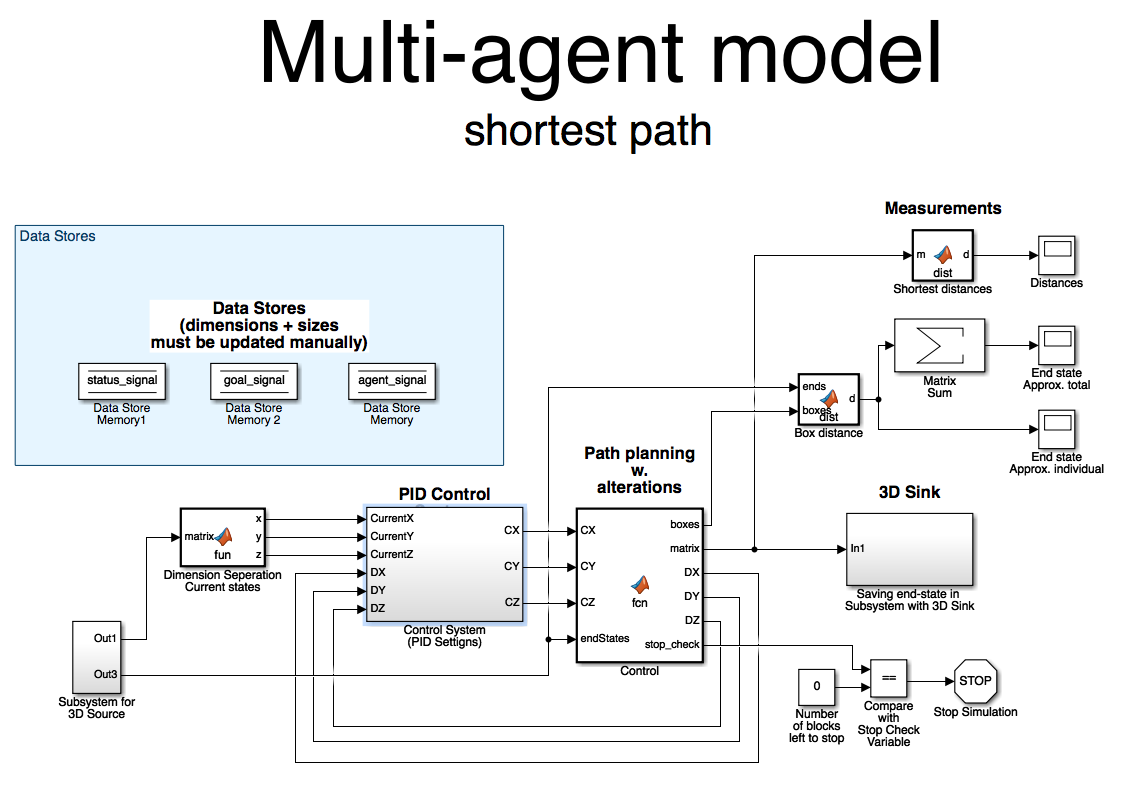
\includegraphics[width=1\columnwidth]{figures/model_overview}
  \caption{\label{fig:model_overview}Overview of finished model in Simulink}
\end{figure}

The following subsections will outline how the different model requirements outlined in Section \ref{sec:physics}, were achieved in a step wise manner.

\subsection{Sources and Sinks}
The simulation is carried out with a start and an endpoint 

\subsection{PID Controller}
\label{sec:sim_pid}

As mentioned in Section \ref{sec:simulation_animation}, it is important the control systems cannot alter the position of the quadcopters directly, but instead gives instructions to the quadcopters to change their thrust etc. 

Force, the parameter that is adjusted to achieve a desired position

base on reference, that PID is used for balancing etc...

\subsection{Gravity \& Mass}
\label{sec:sim_gravity}

\subsection{Control Loop}

\subsection{Data Stores}

\subsection{Measurements}

\subsection{Completion Check}

\section{Validation}
\label{sec:validation}

Validation on single agent level

\subsection{Adjusting for desired behavior}
\label{sec:tuning}

% Pre adjustment
\begin{figure}[H]
  \centering
  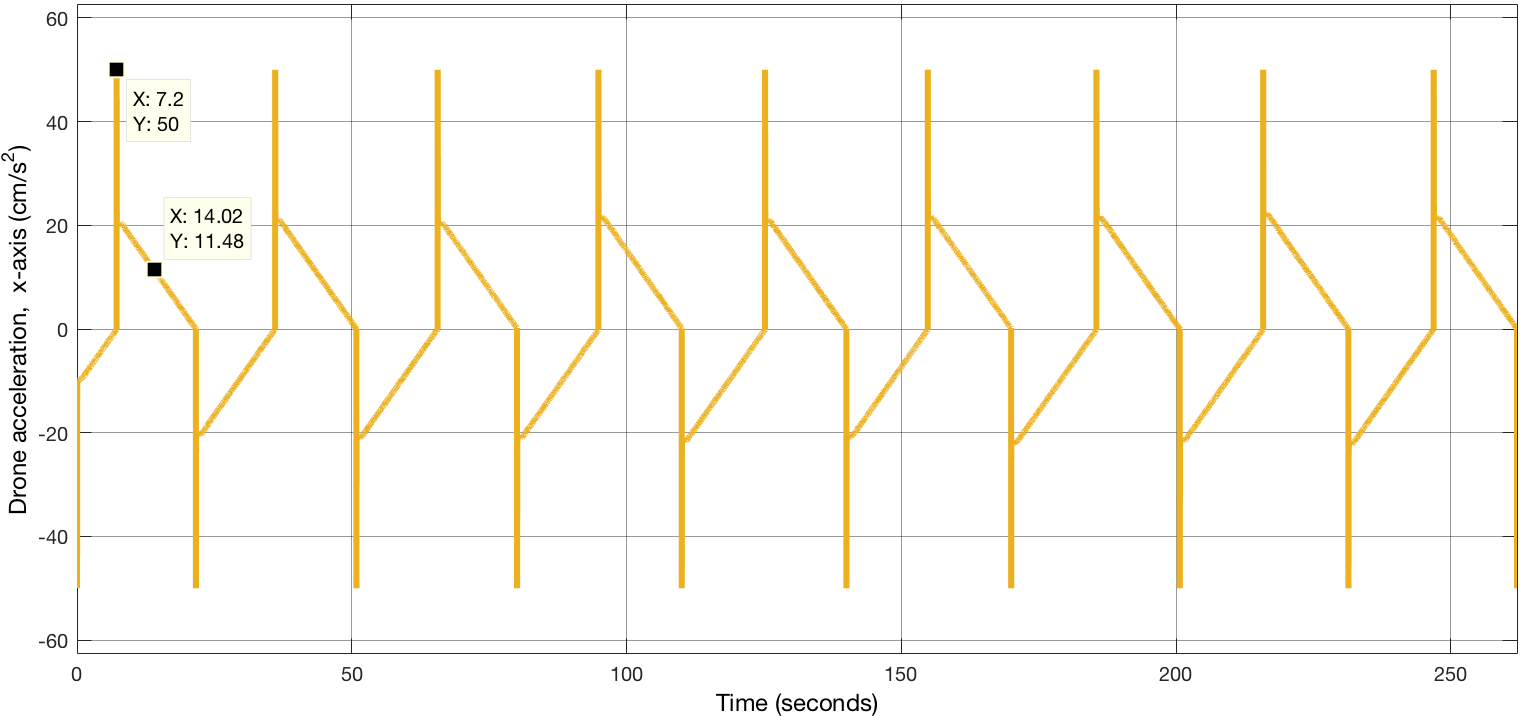
\includegraphics[width=1\columnwidth]{figures/SA_accel_pre_adjustment}
  \caption{\label{fig:pre_adjust}Agent acceleration before adjustment}
\end{figure}

Stable but too tall

% Post adjustment
\begin{figure}[H]
  \centering
  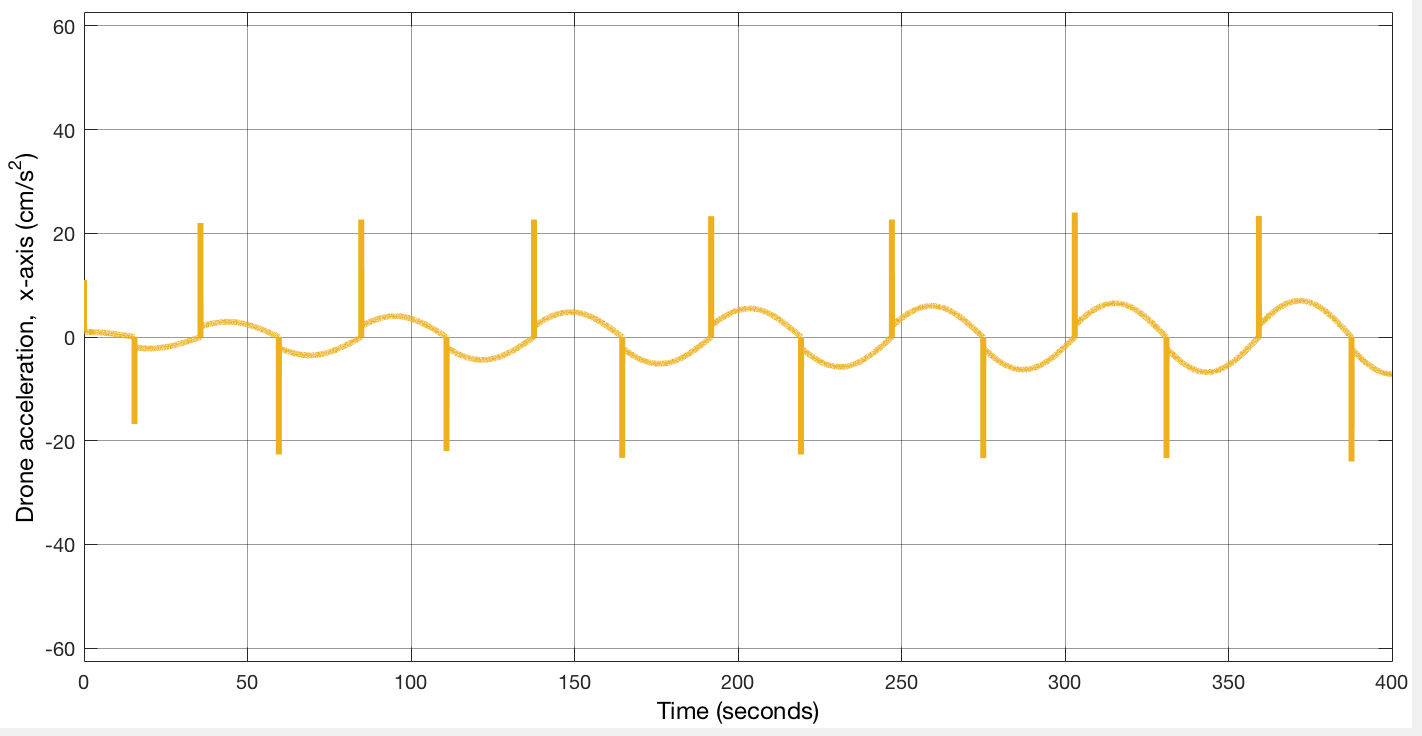
\includegraphics[width=1\columnwidth]{figures/SA_accel_pre_post_p_adjustment}
  \caption{\label{fig:post_adjust}Agent acceleration after adjustment of PD gains}
\end{figure}

short but unstable

% Post limitation
\begin{figure}[H]
  \centering
  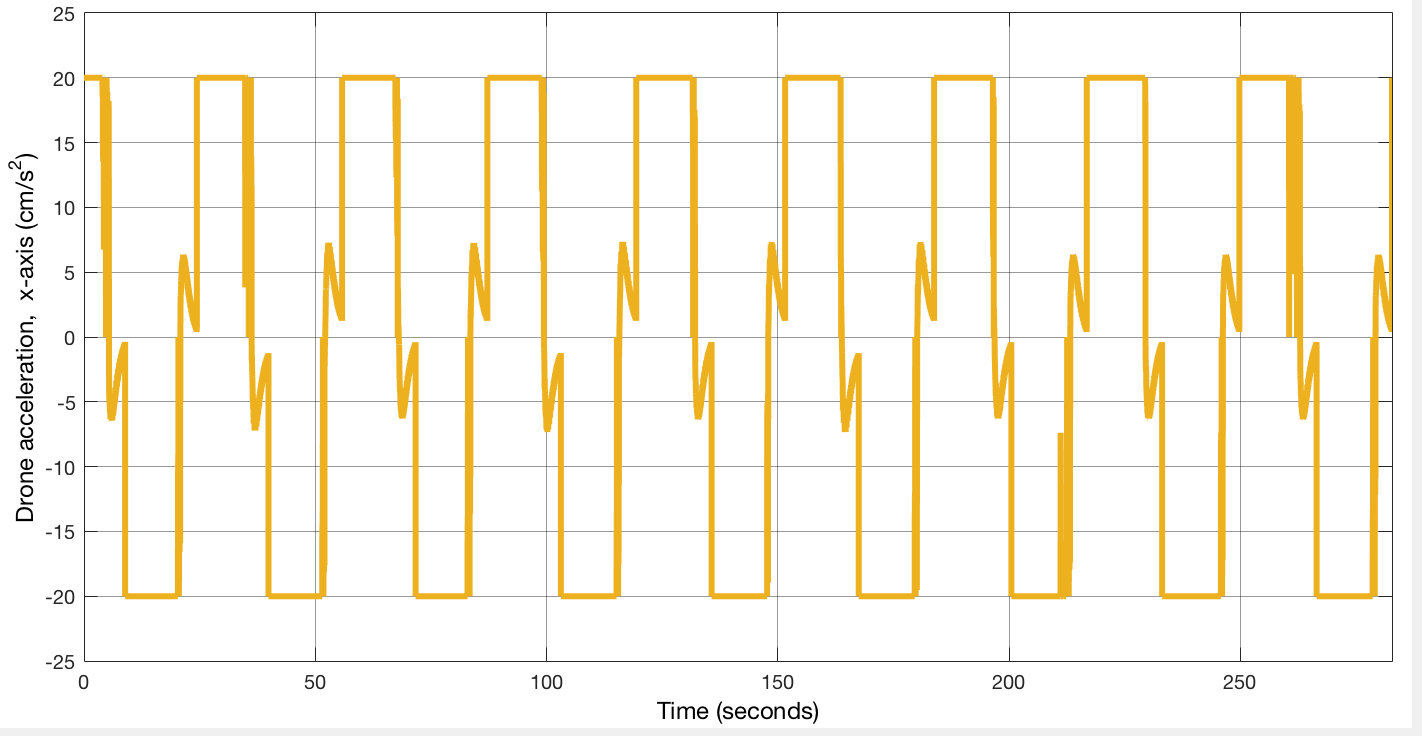
\includegraphics[width=1\columnwidth]{figures/SA_accel_post_final_adjustment}
  \caption{\label{fig:post_limit}Agent acceleration with acceleration}
\end{figure}

Shorter and wider is stable

\section{Test Metrics}
\label{sec:test_metrics}

\subsection{Testing on shortest path}



